%------ VAE performance ------
\subsection{Representation quality}
To understand the generative capabilities of the VAE we show several examples related to shape generation as well as explore the structure of the learned latent space.
Figure~\ref{fig:random_sample} depicts shapes generated by the decoder fed with latent variables randomly sampled from $\mathcal{N}(\bb{0},\bb{I})$. As we have explicitly relaxed the Gaussian prior on the latent variables (small $\lambda$) during training. As discussed earlier, the tradeoff is that samples coming from the prior may generate slightly unrealistic shapes.

Figure \ref{fig:interpolation} depicts generated shapes as the result of linear interpolation in the latent space. The source and target shapes are first passed through the encoder to obtain latent representations; applying the decoder to convex combinations of these latent vectors produces a highly non-linear interpolation in $\mathbb{R}^3$. The top two rows of Figure~\ref{fig:interpolation} show interpolation for networks trained with $\lambda=10^{-6}$ and $\lambda=10^{-8}$, respectively. The bottom row of Figure~\ref{fig:interpolation} highlights the interesting structure of the learned latent space through arithmetic. Applying the difference of a subject with left knee raised and lowered to the same subject with right knee raised results in a lowering of the right knee. The network learned this symmetry without any explicit modeling.


% fig: Random sampling
\begin{figure}
\centering
\includegraphics[height=0.15\textwidth]{./figures/random_sample_6.png}
\includegraphics[height=0.15\textwidth]{./figures/random_sample_13.png}
\includegraphics[height=0.15\textwidth]{./figures/random_sample_14.png}
\includegraphics[height=0.15\textwidth]{./figures/random_sample_15.png}
\includegraphics[height=0.15\textwidth]{./figures/random_sample_22.png}
\includegraphics[height=0.15\textwidth]{./figures/random_sample_30.png}
\includegraphics[height=0.15\textwidth]{./figures/random_sample_59.png}
\includegraphics[height=0.15\textwidth]{./figures/random_sample_66.png}
\includegraphics[height=0.15\textwidth]{./figures/random_sample_70.png}

\caption{\textbf{Random human shapes generated by the VAE.} We have explicitly relaxed the Gaussian prior on the latent variables during training. The tradeoff is that samples coming from the prior may generate slightly unrealistic shapes.}
\label{fig:random_sample}
\end{figure} 
%
\definecolor{mygray}{rgb}{0.6,0.6,0.6}
% fig: interpolation
\begin{figure}
\centering
\resizebox{1\columnwidth}{!}{
\addtolength{\tabcolsep}{-4pt}
\begin{tabular}{cccccc}
\includegraphics[height=0.12\textwidth]{./figures/interp_1e-6_1.png} &
\includegraphics[height=0.12\textwidth]{./figures/interp_1e-6_5.png} &
\includegraphics[height=0.12\textwidth]{./figures/interp_1e-6_9.png} &
\includegraphics[height=0.12\textwidth]{./figures/interp_1e-6_13.png} &
\includegraphics[height=0.12\textwidth]{./figures/interp_1e-6_17.png} &
\includegraphics[height=0.12\textwidth]{./figures/interp_1e-6_19.png} \\
\includegraphics[height=0.12\textwidth]{./figures/interp_1e-8_1.png} &
\includegraphics[height=0.12\textwidth]{./figures/interp_1e-8_5.png} &
\includegraphics[height=0.12\textwidth]{./figures/interp_1e-8_9.png} &
\includegraphics[height=0.12\textwidth]{./figures/interp_1e-8_13.png} &
\includegraphics[height=0.12\textwidth]{./figures/interp_1e-8_17.png} &
\includegraphics[height=0.12\textwidth]{./figures/interp_1e-8_19.png} \\ 
\vspace{10pt} \\
\begin{overpic}
[trim=0cm 0cm 0cm 0cm,clip,height=0.12\textwidth]{./figures/arith_C.png}
\put(12,65){\small Z}
\put(23,65){$+$}
\put(33,65){\small $\alpha$}
\put(41,65){$($}
\end{overpic} &
\begin{overpic}
[trim=0cm 0cm 0cm 0cm,clip,height=0.12\textwidth]{./figures/arith_B.png}
\put(8,65){\small X}
\put(28,65){$ - $}
\end{overpic} &
\begin{overpic}
[trim=0cm 0cm 0cm 0cm,clip,height=0.12\textwidth]{./figures/arith_A.png}
\put(10,65){\small Y}
\put(20,65){$)$}
\put(35,70){ {\color{mygray}\line(0,-1){70}} }
\end{overpic} &
\begin{overpic}
[trim=0cm 0cm 0cm 0cm,clip,height=0.12\textwidth]{./figures/50022_one_leg_jump_00284_12.png}
\put(0,65){\small$\alpha = 0.5$}
\end{overpic} &
\begin{overpic}
[trim=0cm 0cm 0cm 0cm,clip,height=0.12\textwidth]{./figures/50022_one_leg_jump_00284_17.png}
\put(0,65){\small$\alpha = 0.7$}
\end{overpic} &
\begin{overpic}
[trim=0cm 0cm 0cm 0cm,clip,height=0.12\textwidth]{./figures/50022_one_leg_jump_00284_24.png}
\put(0,65){\small $\alpha = 1$}
\end{overpic}
\end{tabular}
}
\caption{\textbf{Latent space interpolation.} Interpolation between two poses (left- and right-most shapes) obtained as convex combinations of the respective representations the the latent space. Bottom row: latent space arithmetic.%All the intermediate poses are plausible. 
%\orlit{top row is 1e-6 and bottom row is 1e-8.}
} 
\label{fig:interpolation}
\end{figure} 
%


%------ Variability ------
\subsection{Completion variability}
\label{subsec:completion_variability}
As explained in Section \ref{sec:method}, given a partial input with more than one solution consistent with the data, we may explore this space of completions by sampling the initialization of problem~\ref{eq:optimization} at random from the Gaussian prior. For evaluation we consider several test subjects with removed limbs. Figure \ref{fig:completion_variability} shows unique plausible completions of the same partial input achieved by random initializations.

\definecolor{mygray}{rgb}{0.6,0.6,0.6}

% fig: Variability
\begin{figure}
%\vspace{3mm}
\centering
\resizebox{1.05\columnwidth}{!}{
%\begin{tabular}{c@{\hskip 0.02\textwidth}c@{\hskip 0.002\textwidth}c@{\hskip 0.002\textwidth}c@{\hskip 0.002\textwidth}c@{\hskip 0.002\textwidth}}
\begin{tabular}{c@{\hskip 5mm}|@{\hskip 5mm}cccc}
%@{\hskip 0.002\textwidth}c@{\hskip 0.002\textwidth}c@{\hskip 0.002\textwidth}c@{\hskip 0.002\textwidth}}
%\begin{overpic}
%[trim=0cm 0cm 0cm 0cm,clip,height=0.20\textwidth]{./figures/both_arms.png}
%\put(2,82){\footnotesize input}
%\put(130,82){\footnotesize completions}
%\put(45,70){ {\color{mygray}\line(0,-1){220}} }
%\end{overpic}
%\hspace{-1mm} & \hspace{2.5mm}
Input & \multicolumn{4}{c}{Completions} \hspace{5mm} \\ \\
\includegraphics[trim=0 0 150 0,clip,height=0.20\textwidth]{./figures/both_arms.png} &
\includegraphics[height=0.20\textwidth]{./figures/both_arms_2.png} &
\includegraphics[height=0.20\textwidth]{./figures/both_arms_1.png} &
\includegraphics[height=0.20\textwidth]{./figures/both_arms_3.png} &
\includegraphics[height=0.20\textwidth]{./figures/both_arms_4.png} \\
\includegraphics[trim=0 0 150 0,clip,height=0.20\textwidth]{./figures/torso.png} &
\includegraphics[height=0.20\textwidth]{./figures/torso_1.png} &
\includegraphics[height=0.20\textwidth]{./figures/torso_2.png} &
\includegraphics[height=0.20\textwidth]{./figures/torso_5.png} &
\includegraphics[height=0.20\textwidth]{./figures/torso_8.png} \\
\includegraphics[trim=0 0 150 0,clip,height=0.20\textwidth]{./figures/torso_limbs.png} &
\includegraphics[height=0.20\textwidth]{./figures/torso_limbs_3.png} & 
\includegraphics[height=0.20\textwidth]{./figures/torso_limbs_4.png} & 
\includegraphics[height=0.20\textwidth]{./figures/torso_limbs_5.png} & 
\includegraphics[height=0.20\textwidth]{./figures/torso_limbs_6.png}
\end{tabular}
}
\caption{\textbf{Completion variability.} When large contiguous regions (e.g. limbs) are missing, the solution to shape completion is not unique. Shown here are different reconstructions with our method obtained using random initializations.
} 
\label{fig:completion_variability}
\end{figure} 

%

%------ Range scan completion ------
\subsection{Synthetic range scans completion}
\label{subsec:range_scans_completion}
%To demonstrate the usefulness of our method, we tested it on what is probably the most common use case, namely, range scans of humans under different articulation. This data is also suitable for qualitative comparison as sufficient information is given in the partial shape to make the completion problem nearly deterministic.
The following experiment considers the common practical scenario of range scan completion.
We utilize a test-set of $200$ virtual scans produced from $10$ viewpoints around $2$ human subjects exhibiting $10$ different poses. The full shapes were taken from FAUST~\cite{Bogo:CVPR:2014}, and are completely disjoint from our train set, as they contain novel subjects and poses. Furthermore, the data is suitable for quantitative comparison as sufficient information is given in the partial shape to make the completion problem nearly deterministic. Keeping the ground truth correspondence from each view to the full shape, we report the mean completion error in table~\ref{tab_proj_completion} as \emph{Ours (ground truth)}. More interesting are the results of end-to-end completion using partial correspondence obtained by MoNet~\cite{monet} (reported as \emph{Ours (MoNet)}). For reference we report the performance of other shape completion methods: 3D-EPN \cite{dai2016shape} which has shown state-of-the-art performance for shape completion using volumetric networks, Poisson reconstruction \cite{kazhdan2013screened}, and nearest neighbor (NN). Note, in order to comply with the architecture of 3D-EPN, we also provide viewpoint information, which is unknown for our method. For NN the completion is considered to be the closest shape from the entire training using the ground truth correspondences. Results in table~\ref{tab_proj_completion} show mean Euclidean distance (in cm) and relative volumetric error (in \%) for the missing region. More results are shown in Figures~\ref{fig:err_matrix} and~\ref{fig:proj_completion}.

\paragraph{Robust optimization.}
Our method is able to generalize well to partial shapes in poses unseen during training. However, there is a gap in performance when using correspondences from an oracle versus an off-the-shelf technique (MoNet). To handle noisy correspondences better, we propose a robust enhancement to (\ref{eq:optimization}). Observing that our method may not converge to the ideal completion if the alignment is guided by poor correspondences. However, if the partial shape is somewhat well aligned with the generated shape we can recalculate the correspondence $\bb{\Pi}$ using a simple Euclidean closest-vertex assignment. We find that recalculating when SGD plateaus leads to improved completions (results are reported in Table~\ref{tab_proj_completion} as \emph{Ours (MoNet with refinement)}).
A pleasant side-effect of this refinement step is that our shape completion method can be used to obtain a de-noised (albeit sparser) set  of correspondences (see the supplemental material for analysis).
We also evaluate shape completion when the optimization steps are capped at 300 (reported as \emph{Ours (MoNet with refinement $300$)}) as opposed to running until convergence. Note, for simplicity we did not explore tuning different aspects of the method (learning rate, different reconstruction losses, etc).

\begin{table}[tb]
\centering
\small
\begin{tabular}{ l@{\hskip 0.01\textwidth}c@{\hskip 0.01\textwidth}c@{\hskip 0.01\textwidth}c@{\hskip 0.01\textwidth}c@{\hskip 0.01\textwidth}c@{\hskip 0.01\textwidth}c@{\hskip 0.01\textwidth}c  }
    \hline\hline
    Error & Euclidean & Volumetric err. \\     
          & distance [cm] & mean $\pm$ std [\%] \\ \hline    
    Poisson \cite{kazhdan2013screened}  & $7.3$ 	& $24.8 \pm 23.2$  \\
    NN   (ground truth)   & $5.4$ 	& $34.01 \pm 9.23$  \\   
    3D-EPN \cite{dai2016shape} & $4.43$ & $89.7 \pm 33.8$  \\        
    {\bf Ours} (MoNet)   & $3.40$ 	& $12.51 \pm 11.1$  \\ 
    {\bf Ours} (MoNet with ref. $300$)   & $3.01$ & $10.00  \pm 8.83$ \\ 
    {\bf Ours} (MoNet with refinement)   & $\textbf{2.84}$ 	& $\textbf{9.24}  \pm \textbf{8.62}$ \\ %\hline
    {\bf Ours} (ground truth)   & $\textbf{2.51}$ 	& $\textbf{7.48} \pm \textbf{5.64}$ \\ \hline \hline 
  \end{tabular}   
  \vspace{2mm}
\caption{\small \textbf{Synthetic range scans completion.} Comparison of different methods with respect to errors in vertex position and shape volume. Our method is evaluated using ground truth and MoNet~\cite{monet} correspondences, as well as with and without refinement (details in Section \ref{subsec:range_scans_completion}).
}
\label{tab_proj_completion}
\end{table}


\begin{figure}
\centering
\includegraphics[width=0.5\columnwidth]{./figures/range_scan_comparison}
%% This file was created by matlab2tikz.
%
%The latest updates can be retrieved from
%  http://www.mathworks.com/matlabcentral/fileexchange/22022-matlab2tikz-matlab2tikz
%where you can also make suggestions and rate matlab2tikz.
%
\definecolor{mycolor1}{rgb}{0.00000,0.44700,0.74100}%
\definecolor{mycolor2}{rgb}{0.85000,0.32500,0.09800}%
%
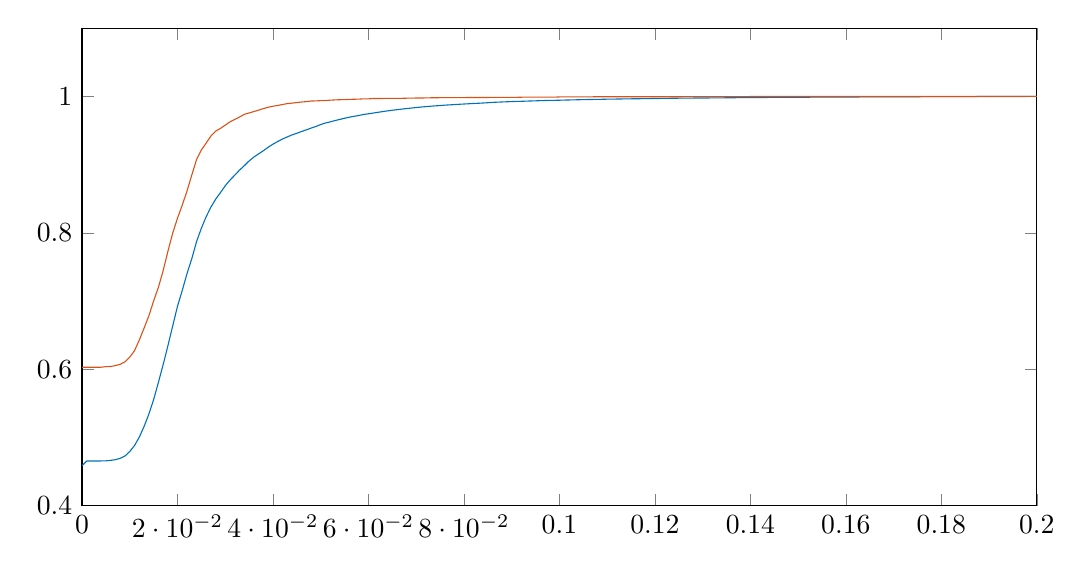
\begin{tikzpicture}

\begin{axis}[%
width=\linewidth,
height=0.5\linewidth,
at={(0.758in,0.481in)},
scale only axis,
xmin=0,
xmax=0.2,
ymin=0.4,
ymax=1.1,
axis background/.style={fill=white}
]
\addplot [color=mycolor1,solid,forget plot]
  table[row sep=crcr]{%
0	0.458519871460353\\
0.001	0.46539035167194\\
0.002	0.465411259635086\\
0.003	0.465411259635086\\
0.004	0.46544610624033\\
0.005	0.465634277908646\\
0.006	0.466331210013521\\
0.007	0.467292976318247\\
0.008	0.46932801806448\\
0.009	0.472708138773121\\
0.01	0.479342932411525\\
0.011	0.488054583722454\\
0.012	0.500515729757607\\
0.013	0.516001561127915\\
0.014	0.534073010607307\\
0.015	0.555503672832193\\
0.016	0.580704737744449\\
0.017	0.606853630319334\\
0.018	0.634723945193259\\
0.019	0.663611780940301\\
0.02	0.692374168908465\\
0.021	0.715651701211268\\
0.022	0.740413698897454\\
0.023	0.762185857853728\\
0.024	0.787296321592351\\
0.025	0.80676860460254\\
0.026	0.823578606972109\\
0.027	0.837698451416863\\
0.028	0.849434788062947\\
0.029	0.858947911294482\\
0.03	0.86899767224677\\
0.031	0.877381765468408\\
0.032	0.884553196827565\\
0.033	0.891940677139233\\
0.034	0.898491838925052\\
0.035	0.905412374726454\\
0.036	0.911057524775937\\
0.037	0.915733939199643\\
0.038	0.920445200228594\\
0.039	0.925484019346836\\
0.04	0.929986200744324\\
0.041	0.933854173926376\\
0.042	0.937589730008503\\
0.043	0.940607446022609\\
0.044	0.94359728475252\\
0.045	0.945952915266995\\
0.046	0.948608226586566\\
0.047	0.950956887779993\\
0.048	0.95357735249432\\
0.049	0.955974798935088\\
0.05	0.958741619391439\\
0.051	0.961027556695427\\
0.052	0.962721101710272\\
0.053	0.964609787714481\\
0.054	0.966268486124082\\
0.055	0.968003847065219\\
0.056	0.969488312448602\\
0.057	0.97088217665835\\
0.058	0.972066961236637\\
0.059	0.973551426620019\\
0.06	0.974541070208941\\
0.061	0.975593437687301\\
0.062	0.976694590413002\\
0.063	0.977774835175558\\
0.064	0.978785386727625\\
0.065	0.979740183711303\\
0.066	0.980562563595055\\
0.067	0.981377974157758\\
0.068	0.98220035404151\\
0.069	0.982925163430579\\
0.07	0.983705727388038\\
0.071	0.984409628813961\\
0.072	0.9850298983873\\
0.073	0.985594413392248\\
0.074	0.986144989755099\\
0.075	0.986584056981169\\
0.076	0.987197357233459\\
0.077	0.987594608533237\\
0.078	0.988040645080357\\
0.079	0.98846577366433\\
0.08	0.988849086322011\\
0.081	0.989239368300741\\
0.082	0.989650558242617\\
0.083	0.989950239047713\\
0.084	0.990333551705393\\
0.085	0.990758680289367\\
0.086	0.991260471404876\\
0.087	0.99157409085207\\
0.088	0.991873771657166\\
0.089	0.992138605857018\\
0.09	0.992445255983163\\
0.091	0.992654335614625\\
0.092	0.992828568640844\\
0.093	0.99307249487755\\
0.094	0.993309451793207\\
0.095	0.99351156210362\\
0.096	0.993783365624521\\
0.097	0.993971537292837\\
0.098	0.994138800998007\\
0.099	0.994250310134787\\
0.1	0.994410604518908\\
0.101	0.994619684150371\\
0.102	0.99478694785554\\
0.103	0.994947242239662\\
0.104	0.995128444586929\\
0.105	0.995281769650001\\
0.106	0.995428125392025\\
0.107	0.995546603849854\\
0.108	0.995672051628731\\
0.109	0.995776591444462\\
0.11	0.995957793791729\\
0.111	0.996055364286412\\
0.112	0.996145965460045\\
0.113	0.996264443917874\\
0.114	0.996375953054654\\
0.115	0.996487462191434\\
0.116	0.996598971328214\\
0.117	0.996654725896604\\
0.118	0.996752296391286\\
0.119	0.996856836207017\\
0.12	0.996926529417505\\
0.121	0.997017130591138\\
0.122	0.997128639727918\\
0.123	0.997219240901552\\
0.124	0.997281964790991\\
0.125	0.997393473927771\\
0.126	0.997449228496161\\
0.127	0.997546798990843\\
0.128	0.997595584238184\\
0.129	0.997679216090769\\
0.13	0.997707093374964\\
0.131	0.997734970659159\\
0.132	0.997776786585452\\
0.133	0.997853449116988\\
0.134	0.997909203685378\\
0.135	0.99800677418006\\
0.136	0.998069498069499\\
0.137	0.99811828331684\\
0.138	0.998208884490474\\
0.139	0.998236761774669\\
0.14	0.998292516343058\\
0.141	0.998348270911448\\
0.142	0.998390086837741\\
0.143	0.998438872085082\\
0.144	0.998522503937667\\
0.145	0.998543411900813\\
0.146	0.998613105111301\\
0.147	0.998647951716544\\
0.148	0.998689767642837\\
0.149	0.998724614248081\\
0.15	0.998759460853324\\
0.151	0.998808246100665\\
0.152	0.998815215421714\\
0.153	0.998884908632202\\
0.154	0.998905816595348\\
0.155	0.998933693879543\\
0.156	0.998968540484786\\
0.157	0.998982479126884\\
0.158	0.999010356411079\\
0.159	0.999045203016323\\
0.16	0.999100957584713\\
0.161	0.999142773511005\\
0.162	0.999177620116249\\
0.163	0.99922640536359\\
0.164	0.999261251968834\\
0.165	0.99928215993198\\
0.166	0.999303067895126\\
0.167	0.999344883821419\\
0.168	0.999372761105613\\
0.169	0.999386699747711\\
0.17	0.999428515674003\\
0.171	0.99944942363715\\
0.172	0.999498208884491\\
0.173	0.999546994131832\\
0.174	0.99956093277393\\
0.175	0.999567902094978\\
0.176	0.999595779379173\\
0.177	0.999609718021271\\
0.178	0.999630625984417\\
0.179	0.999651533947563\\
0.18	0.999658503268612\\
0.181	0.99967244191071\\
0.182	0.999686380552807\\
0.183	0.999707288515953\\
0.184	0.9997281964791\\
0.185	0.999749104442246\\
0.186	0.999770012405392\\
0.187	0.99978395104749\\
0.188	0.999811828331685\\
0.189	0.999818797652733\\
0.19	0.99983970561588\\
0.191	0.999853644257977\\
0.192	0.999853644257977\\
0.193	0.999867582900075\\
0.194	0.999881521542172\\
0.195	0.999888490863221\\
0.196	0.999923337468465\\
0.197	0.999923337468465\\
0.198	0.999951214752659\\
0.199	0.999986061357903\\
0.2	1\\
};
\addplot [color=mycolor2,solid,forget plot]
  table[row sep=crcr]{%
0	0.602742371572036\\
0.001	0.602917028880518\\
0.002	0.602917028880518\\
0.003	0.602917028880518\\
0.004	0.602917028880518\\
0.005	0.603689751762774\\
0.006	0.60397952284362\\
0.007	0.605331787887569\\
0.008	0.607167004732928\\
0.009	0.610837438423645\\
0.01	0.61769535400367\\
0.011	0.627161209311311\\
0.012	0.642808847677002\\
0.013	0.660291702888052\\
0.014	0.678257509900512\\
0.015	0.700086931324254\\
0.016	0.720081135902637\\
0.017	0.744711677774558\\
0.018	0.773205834057761\\
0.019	0.799671592775041\\
0.02	0.821597604559065\\
0.021	0.840625905534628\\
0.022	0.861489423355549\\
0.023	0.884864290543804\\
0.024	0.907659615570366\\
0.025	0.921472037090698\\
0.026	0.931517434560031\\
0.027	0.941949193470492\\
0.028	0.949096880131363\\
0.029	0.953153675263209\\
0.03	0.957886602917029\\
0.031	0.962716120931131\\
0.032	0.966193373901285\\
0.033	0.969863807592002\\
0.034	0.973727422003284\\
0.035	0.975755819569207\\
0.036	0.97778421713513\\
0.037	0.979909205061335\\
0.038	0.982130783347822\\
0.039	0.984159180913745\\
0.04	0.985608036317975\\
0.041	0.98676712064136\\
0.042	0.988119385685308\\
0.043	0.989471650729257\\
0.044	0.990147783251231\\
0.045	0.99101709649377\\
0.046	0.991789819376026\\
0.047	0.992369361537718\\
0.048	0.993238674780257\\
0.049	0.993431855500821\\
0.05	0.993818216941949\\
0.051	0.993914807302231\\
0.052	0.994494349463923\\
0.053	0.994880710905051\\
0.054	0.995170481985898\\
0.055	0.99526707234618\\
0.056	0.995653433787308\\
0.057	0.995846614507872\\
0.058	0.996039795228436\\
0.059	0.996426156669564\\
0.06	0.996426156669564\\
0.061	0.996909108470974\\
0.062	0.996909108470974\\
0.063	0.997005698831256\\
0.064	0.997102289191539\\
0.065	0.997102289191539\\
0.066	0.997198879551821\\
0.067	0.997198879551821\\
0.068	0.997392060272385\\
0.069	0.997392060272385\\
0.07	0.997681831353231\\
0.071	0.997681831353231\\
0.072	0.997778421713513\\
0.073	0.997971602434077\\
0.074	0.997971602434077\\
0.075	0.998164783154641\\
0.076	0.998164783154641\\
0.077	0.998261373514923\\
0.078	0.998261373514923\\
0.079	0.998261373514923\\
0.08	0.998261373514923\\
0.081	0.998454554235487\\
0.082	0.998454554235487\\
0.083	0.998454554235487\\
0.084	0.998454554235487\\
0.085	0.998454554235487\\
0.086	0.998551144595769\\
0.087	0.998551144595769\\
0.088	0.998551144595769\\
0.089	0.998647734956051\\
0.09	0.998647734956051\\
0.091	0.998647734956051\\
0.092	0.998840915676615\\
0.093	0.998937506036898\\
0.094	0.998937506036898\\
0.095	0.998937506036898\\
0.096	0.998937506036898\\
0.097	0.998937506036898\\
0.098	0.998937506036898\\
0.099	0.998937506036898\\
0.1	0.999227277117744\\
0.101	0.999227277117744\\
0.102	0.999227277117744\\
0.103	0.999227277117744\\
0.104	0.999420457838308\\
0.105	0.999420457838308\\
0.106	0.999420457838308\\
0.107	0.999420457838308\\
0.108	0.99951704819859\\
0.109	0.99951704819859\\
0.11	0.99951704819859\\
0.111	0.99951704819859\\
0.112	0.99951704819859\\
0.113	0.99951704819859\\
0.114	0.99951704819859\\
0.115	0.99951704819859\\
0.116	0.99951704819859\\
0.117	0.99951704819859\\
0.118	0.99951704819859\\
0.119	0.99951704819859\\
0.12	0.99951704819859\\
0.121	0.99951704819859\\
0.122	0.99951704819859\\
0.123	0.99951704819859\\
0.124	0.99951704819859\\
0.125	0.99951704819859\\
0.126	0.999613638558872\\
0.127	0.999613638558872\\
0.128	0.999613638558872\\
0.129	0.999613638558872\\
0.13	0.999613638558872\\
0.131	0.999710228919154\\
0.132	0.999710228919154\\
0.133	0.999710228919154\\
0.134	0.999710228919154\\
0.135	0.999710228919154\\
0.136	0.999710228919154\\
0.137	0.999710228919154\\
0.138	0.999710228919154\\
0.139	0.999710228919154\\
0.14	0.999806819279436\\
0.141	0.999806819279436\\
0.142	0.999806819279436\\
0.143	0.999806819279436\\
0.144	0.999806819279436\\
0.145	0.999806819279436\\
0.146	0.999806819279436\\
0.147	0.999806819279436\\
0.148	0.999806819279436\\
0.149	0.999806819279436\\
0.15	0.999806819279436\\
0.151	0.999806819279436\\
0.152	0.999806819279436\\
0.153	0.999806819279436\\
0.154	0.999806819279436\\
0.155	0.999806819279436\\
0.156	0.999806819279436\\
0.157	0.999806819279436\\
0.158	0.999806819279436\\
0.159	0.999806819279436\\
0.16	0.999806819279436\\
0.161	0.999903409639718\\
0.162	0.999903409639718\\
0.163	0.999903409639718\\
0.164	0.999903409639718\\
0.165	0.999903409639718\\
0.166	0.999903409639718\\
0.167	0.999903409639718\\
0.168	0.999903409639718\\
0.169	0.999903409639718\\
0.17	0.999903409639718\\
0.171	0.999903409639718\\
0.172	0.999903409639718\\
0.173	0.999903409639718\\
0.174	0.999903409639718\\
0.175	0.999903409639718\\
0.176	0.999903409639718\\
0.177	0.999903409639718\\
0.178	0.999903409639718\\
0.179	0.999903409639718\\
0.18	0.999903409639718\\
0.181	0.999903409639718\\
0.182	0.999903409639718\\
0.183	0.999903409639718\\
0.184	0.999903409639718\\
0.185	0.999903409639718\\
0.186	0.999903409639718\\
0.187	0.999903409639718\\
0.188	1\\
0.189	1\\
0.19	1\\
0.191	1\\
0.192	1\\
0.193	1\\
0.194	1\\
0.195	1\\
0.196	1\\
0.197	1\\
0.198	1\\
0.199	1\\
0.2	1\\
};
\end{axis}
\end{tikzpicture}%
\caption{\textbf{Reconstruction error as a function of view angle.} Our method produces a consistently accurate reconstruction independent of the view angle. } 
\label{fig:err_matrix}
\end{figure} 

% \begin{figure}
% \centering
% %\vspace{12pt}
% \resizebox{1.05\columnwidth}{!}{
% \addtolength{\tabcolsep}{-4pt}
% \begin{tabular}{cccccc}
% \begin{overpic}
% [trim=0cm 0cm 0cm 0cm,clip,height=0.165\textwidth]{./figures/proj_part.png}
% \put(0,88){\small input}
% \end{overpic} & 
% \begin{overpic}
% [trim=0cm 0cm 0cm 0cm,clip,height=0.165\textwidth]{./figures/proj_full.png}
% \put(-7,88){\small ground truth}
% \end{overpic} & 
% \begin{overpic}
% [trim=0cm 0cm 0cm 0cm,clip,height=0.165\textwidth]{./figures/proj_poiss_recon.png}
% \put(-5,88){\small Poisson}
% \end{overpic} & 
% \begin{overpic}
% [trim=0cm 0cm 0cm 0cm,clip,height=0.165\textwidth]{./figures/proj_NN_recon.png}
% \put(0,88){\small NN}
% \end{overpic} & 
% \begin{overpic}
% [trim=0cm 0cm 0cm 0cm,clip,height=0.165\textwidth]{./figures/proj_voxnet_recon.png}
% \put(-7,88){\small 3D-EPN}
% \end{overpic} & 
% \begin{overpic}
% [trim=0cm 0cm 0cm 0cm,clip,height=0.165\textwidth]{./figures/proj_ours_recon.png}
% \put(3,88){\small Ours}
% \end{overpic} \vspace{2mm}\\ 
% \includegraphics[height=0.15\textwidth]{./figures/proj_99_5_part.png} &
% \includegraphics[height=0.15\textwidth]{./figures/proj_99_5_full.png} &
% \includegraphics[height=0.15\textwidth]{./figures/proj_99_5_poiss_recon.png} &
% \includegraphics[height=0.15\textwidth]{./figures/proj_99_5_NN_recon.png} &
% \includegraphics[height=0.15\textwidth]{./figures/proj_99_5_voxnet_recon.png} &
% \includegraphics[height=0.15\textwidth]{./figures/proj_99_5_ours_recon.png}
% %  & \includegraphics[height=0.15\textwidth]{./figures/colorbar.eps} %& \includegraphics[height=0.15\textwidth]{./figures/ptwise_err_poiss.png} & \includegraphics[height=0.15\textwidth]{./figures/ptwise_err_nn.png} %&
% %\includegraphics[height=0.15\textwidth]{./figures/ptwise_err_voxnet.png} & 
% %\includegraphics[height=0.15\textwidth]%{./figures/ptwise_err_ours.png} 
% \end{tabular}
% }
% \vspace{2mm}
% \caption{\textbf{Comparison of different synthetic range scan completion methods.} Depicted left-to-right: input range scan, ground truth complete shape, Poisson reconstruction, 3D-EPN, and our method. 
% %Bottom row shows pointwise errors between the ground truth and the completed shapes on the unseen parts.
% } 
% \label{fig:proj_completion}
% \end{figure} 

\begin{figure*}
\centering
%\vspace{12pt}
%\resizebox{1.85\columnwidth}{!}{
\addtolength{\tabcolsep}{-4pt}
\begin{tabular}{c@{\hskip 7mm}c@{\hskip 7mm}c@{\hskip 7mm}c@{\hskip 7mm}c@{\hskip 7mm}c}
Input & Ground truth & Poisson & NN & 3D-EPN & Ours \\ \\
\includegraphics[trim=0 0 75 0,clip,height=0.18\textwidth]{./figures/proj_part.png} &
\includegraphics[trim=0 0 75 0,clip,height=0.18\textwidth]{./figures/proj_full.png} &
\includegraphics[trim=0 0 75 0,clip,height=0.18\textwidth]{./figures/proj_poiss_recon.png} &
\includegraphics[trim=0 0 75 0,clip,height=0.18\textwidth]{./figures/proj_NN_recon.png} &
\includegraphics[trim=0 0 75 0,clip,height=0.18\textwidth]{./figures/proj_voxnet_recon.png} &
\includegraphics[trim=0 0 75 0,clip,height=0.18\textwidth]{./figures/proj_ours_recon.png} \\ 
\includegraphics[trim=0 0 75 0,clip,height=0.18\textwidth]{./figures/proj_99_5_part.png} &
\includegraphics[trim=0 0 75 0,clip,height=0.18\textwidth]{./figures/proj_99_5_full.png} &
\includegraphics[trim=0 0 75 0,clip,height=0.18\textwidth]{./figures/proj_99_5_poiss_recon.png} &
\includegraphics[trim=0 0 75 0,clip,height=0.18\textwidth]{./figures/proj_99_5_NN_recon.png} &
\includegraphics[trim=0 0 75 0,clip,height=0.18\textwidth]{./figures/proj_99_5_voxnet_recon.png} &
\includegraphics[trim=0 0 75 0,clip,height=0.18\textwidth]{./figures/proj_99_5_ours_recon.png}
\end{tabular}
%}
\caption{\textbf{Comparison of different synthetic range scan completion methods.} From left to right: input range scan, ground truth complete shape, Poisson reconstruction, 3D-EPN, and our method. 
%Bottom row shows pointwise errors between the ground truth and the completed shapes on the unseen parts.
} 
\label{fig:proj_completion}
\end{figure*} 

% \begin{figure}
% \centering
% \includegraphics[width=0.35\textwidth]{./figures/refine_monet.eps}
% \caption{\textbf{Correspondence refinement.}
% %\orlit{TBD}
% } 
% \label{fig:monet_refine}
% \end{figure}

%------ Dynamic Fusion ------
\subsection{Dynamic Fusion}
\label{subsec:dynamic_fusion}

A common use case of depth scanners is object reconstruction form multiple viewpoints. For static scenes, this problem was explored extensively, e.g., in \cite{newcombe2011kinectfusion,niessner2013real,endres2012evaluation}. Non-rigid deformations pose a much bigger challenge. The works of \cite{newcombe2015dynamicfusion} and \cite{innmann2016volumedeform} have shown very impressive reconstructions, however they are limited to small motions between consecutive frames. This limitation was addressed in \cite{slavcheva2017killingfusion} by introducing a damped Killing motion constraint. These methods are focused on reconstructing only the observed dynamic surfaces and cannot convincingly hallucinate large unseen regions. 
Having developed a completion method for non-rigid shapes, we propose its extension to multiple partial inputs. Registering the partial inputs, or the individual reconstructed shapes, is challenging. Instead, we propose to merge shapes in the latent space: we obtain $\bb{z}$ by averaging the completed shape latent variables for each partial input, and $\mathrm{dec}(\bb{z})$ produces the fused 3D shape. Since the latent representation mixes body shape and pose, the reconstructed pose will generally not adhere to any of the input poses, but rather will be an interpolation thereof. 

For a quantitative analysis, we perform fusion on three partial views from a static shape. We use the same FAUST shapes used for testing in Section \ref{subsec:range_scans_completion}. Table~\ref{tab:static_fusion} shows mean reconstruction errors for all $20$ test shapes when fusing three different partial views. The results show how reconstruction accuracy changes according to the viewpoint, and consistently improves with latent space fusion. A qualitative evaluation of the fusion problem is shown for the dynamic setting in Figure~\ref{fig:dynamic_fusion}. Each row shows three partial views of the same human subject from a different viewpoint \emph{and} a different pose. The latent space fusion of the completed shapes is shown in column 4. %and for comparison the human subject in a canonical pose is shown in the final column.   
%\orlit{TBD} 


%--- tab: rigid fusion
\begin{table}[tb]
\centering
\small
\begin{tabular}{ c c c c }
    \hline\hline
     View 1 & View 2 & View 3 & Fused  \\ \hline  
     $2.78$ & $2.94$ & $2.93$ & $\textbf{2.59}$ \\
     $3.03$ & $3.39$ & $2.73$ & $\textbf{2.61}$ \\ 
     \hline \hline 
\end{tabular}   
  \vspace{2mm}

\caption{\small \textbf{Fusion in the latent space.}
Reported is the mean Euclidean error in cm for three partial views ($0^o$, $120^o$ and $240^o$ for the first row and $80^o$, $200^o$ and $320^o$ for the second row). 
}

\label{tab:static_fusion}
\end{table}



%--- fig: dynamic fusion
\begin{figure}
\centering
\resizebox{0.9\columnwidth}{!}{
\addtolength{\tabcolsep}{-4pt}
\begin{tabular}{cccc}
%{\footnotesize pose 1, view 1} & {\footnotesize pose 2, view 2} & {\footnotesize pose 10, view 7} & {\footnotesize fused} %\\
\includegraphics[height=0.25\textwidth]{./figures/scan_1_80_3.png} &
\includegraphics[height=0.25\textwidth]{./figures/scan_1_81_5.png} &
\includegraphics[height=0.25\textwidth]{./figures/scan_1_89_7.png} &
\includegraphics[height=0.25\textwidth]{./figures/fuse_1.png} \\
%\includegraphics[width=0.2\textwidth]{./figures/canonical_80.png} \\
%pose 1, view 4 & pose 2, view 7 & pose 10, view 10 & fused %\\
\includegraphics[height=0.25\textwidth]{./figures/scan_5_90_4.png} &
\includegraphics[height=0.25\textwidth]{./figures/scan_5_91_7.png} &
\includegraphics[height=0.25\textwidth]{./figures/scan_5_99_10.png} &
\includegraphics[height=0.25\textwidth]{./figures/fuse_5.png}
%\includegraphics[width=0.2\textwidth]{./figures/canonical_90.png} \\
\end{tabular}
}
\vspace{3mm}
\caption{\textbf{Dynamic fusion.} Three partial views (columns 1-3) and the reconstructed complete shape (rightmost column).} 
\label{fig:dynamic_fusion}
\end{figure} 

%------ Real data experiment ------
\subsection{Real range scan completion}
The MHAD dataset \cite{ofli2013berkeley} provides Kinect scans from $2$ viewpoints of subjects performing a variety of actions. We apply our completion method to the extracted point cloud (correspondences were initialized through coarse alignment to a training shape, see the supplemental for details). Figure \ref{fig:err_real_data} depicts examples of scan completion on the Kinect data as well as on real scans from the DFAUST dataset.

\begin{figure}
\centering
\resizebox{0.95\columnwidth}{!}{
\begin{tabular}{ccc}
\includegraphics[height=0.3\textwidth]{./figures/mhad_depth.png} &
\includegraphics[height=0.3\textwidth]{./figures/mhad_pc.png} &
\includegraphics[trim=0 0 40 0,clip,height=0.3\textwidth]{./figures/mhad_recon_1.png} \\
\includegraphics[height=0.3\textwidth]{./figures/mhad_depth_3.png} &
\includegraphics[height=0.3\textwidth]{./figures/mhad_pc_3.png} &
\includegraphics[trim=0 0 40 0,clip,height=0.3\textwidth]{./figures/mhad_recon_3.png}
\end{tabular}
}
\newline
\resizebox{0.95\columnwidth}{!}{
\begin{tabular}{cc@{\hskip 15mm}cc}
\includegraphics[height=0.3\textwidth]{./figures/real_scan_dfaust_50022_knees.png} &
\includegraphics[trim=0 0 40 0,clip,height=0.3\textwidth]{./figures/real_scan_dfaust_50022_knees_recon.png} &
\includegraphics[height=0.3\textwidth] {./figures/real_scan_dfaust_50026_shake_arms.png} &
\includegraphics[trim=0 0 40 0,clip,height=0.3\textwidth]{./figures/real_scan_dfaust_50026_shake_arms_recon.png}
\end{tabular}
}
\caption{\textbf{Completion of real range scans.} First two rows: completion of Kinect scans (left: depth image; middle: extracted point cloud; right: completed shape). Last row: completion of scans from the DFAUST dataset.
\vspace{-2mm}
} 
\label{fig:err_real_data}
\end{figure} 

%------ Non-human experiment ------
\subsection{Face completion}
\label{sec:facecompletion}
A strength of our fully data-driven approach is that by avoiding explicit shape modeling it generalizes easily to different classes of shapes. This is illustrated by an evaluation on deformable faces. $2000$ training face meshes, each with $525$ vertices, are generated from the model provided by \cite{gerig2017morphable}. These face models exhibit less variability in pose relative to the human meshes, so we use a much smaller VAE network (only two convolutional layers and a latent dimensionality of $32$). Figure~\ref{fig:faces} shows completion for different styles of simulated partiality as well as simulated correspondence noise (see the supplemental for more details).

\begin{figure}%[tbh]
\centering
%\addtolength{\tabcolsep}{-4pt}
\resizebox{0.95\columnwidth}{!}{
\begin{tabular}{cccc}
\includegraphics[width=0.11\textwidth]{./figures/part_00.png} &
\includegraphics[width=0.11\textwidth]{./figures/part_03.png} &
\includegraphics[width=0.10\textwidth]{./figures/part_11.png} &
\includegraphics[width=0.11\textwidth]{./figures/part_19.png} \\

\includegraphics[width=0.11\textwidth]{./figures/recon_00.png} &
\includegraphics[width=0.11\textwidth]{./figures/recon_03.png} &
\includegraphics[width=0.11\textwidth]{./figures/recon_11.png} &
\includegraphics[width=0.11\textwidth]{./figures/recon_19.png} \\ \\

\includegraphics[width=0.11\textwidth]{./figures/face_hyp_part_01.png} &
\includegraphics[width=0.09\textwidth]{./figures/face_hyp_part_02.png} &
\includegraphics[width=0.11\textwidth]{./figures/face_hyp_part_07.png} &
\includegraphics[width=0.11\textwidth]{./figures/face_hyp_part_12.png} \\

\includegraphics[width=0.11\textwidth]{./figures/face_hyp_recon_01.png} &
\includegraphics[width=0.11\textwidth]{./figures/face_hyp_recon_02.png} &
\includegraphics[width=0.11\textwidth]{./figures/face_hyp_recon_07.png} &
\includegraphics[width=0.11\textwidth]{./figures/face_hyp_recon_12.png} \\ \\

\includegraphics[width=0.11\textwidth]{./figures/face_n5_part_01.png} &
\includegraphics[width=0.11\textwidth]{./figures/face_n5_part_02.png} &
\includegraphics[width=0.11\textwidth]{./figures/face_n5_part_09.png} &
\includegraphics[width=0.11\textwidth]{./figures/face_n5_part_10.png} \\ 

\includegraphics[width=0.11\textwidth]{./figures/face_n5_recon_01.png} &
\includegraphics[width=0.11\textwidth]{./figures/face_n5_recon_02.png} &
\includegraphics[width=0.11\textwidth]{./figures/face_n5_recon_09.png} &
\includegraphics[width=0.11\textwidth]{./figures/face_n5_recon_10.png} \\ \\

\includegraphics[width=0.11\textwidth]{./figures/face_n30_part_00.png} &
\includegraphics[width=0.06\textwidth]{./figures/face_n30_part_01.png} &
\includegraphics[width=0.11\textwidth]{./figures/face_n30_part_08.png} &
\includegraphics[width=0.11\textwidth]{./figures/face_n30_part_09.png} \\ 

\includegraphics[width=0.11\textwidth]{./figures/face_n30_recon_00.png} &
\includegraphics[width=0.11\textwidth]{./figures/face_n30_recon_01.png} &
\includegraphics[width=0.11\textwidth]{./figures/face_n30_recon_08.png} &
\includegraphics[width=0.11\textwidth]{./figures/face_n30_recon_09.png}
\end{tabular}
}
\caption{{\bf Completion of faces.} Inputs and outputs are shown in the odd and even rows, respectively.
Rows 1-2 show completion for missing patches, rows 3-4 show completion for hyperplane cuts, rows 5-6 show completion for hyperplane cuts and 5\% correspondence error, and rows 7-8 show 30\% correspondence error. Results indicate completion is plausible even under large missing regions and robust to reasonable correspondence error.}
\label{fig:faces}
\end{figure} 